\documentclass[fontsize=14pt]{scrartcl}
\usepackage[landscape,a4paper,left=2cm,right=2cm,top=2cm,bottom=2cm]{geometry}
\usepackage{pdflscape,setspace,amsmath,amssymb}
\usepackage[utf8]{inputenc}
\usepackage[portuguese]{babel}
\usepackage[T1]{fontenc}
\usepackage{tgpagella}
\usepackage{graphicx}
\usepackage[pages=all]{background}
\backgroundsetup{
scale=1,
angle=0,
opacity=1,
position={12.4cm,-7.9cm},
contents={%
  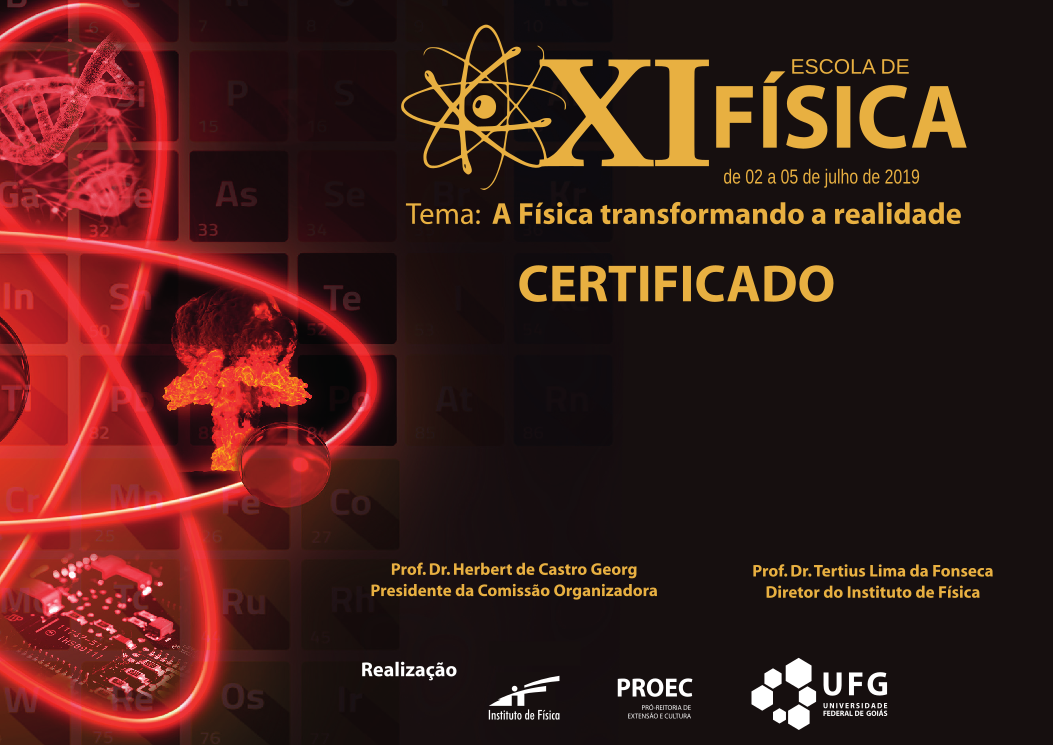
\includegraphics[width=30cm]{background.png}
  }%
}

\begin{document}
\thispagestyle{empty}
\vspace*{7.5cm}
\hspace{7cm}
\begin{minipage}[t][7cm][t]{19cm}
%\doublespacing
\normalfont \bfseries
\textcolor{white}{A Comissão Organizadora certifica que varNOME assistiu ao minicurso intitulado ``varCURSO'' na \mbox{XI} \mbox{Escola} de \mbox{Física}, realizada de 02 a 05 de julho de 2019 no Instituto do Física da Universidade Federal de Goiás, com carga horária de varHORAS horas de atividades}.
\end{minipage}
\end{document} 